\section{三大抽样分布}

\subsection{\texorpdfstring{$\chi^2$}. 分布}

\begin{definition}[卡方分布]
    设 $ X_{1}, X_{2}, \cdots, X_{n} $ 相互独立, 且都服从标准正态分布 $ N(0,1) $, 则称统计量
    $$\chi^{2}=X_{1}^{2}+X_{2}^{2}+\cdots+X_{n}^{2}$$
    服从自由度为 $ n $ 的 $ \chi^{2} $ 分布, 记为 $ \chi^{2} \sim \chi^{2}(n) .$
\end{definition}

\begin{figure}[H]
    \centering
    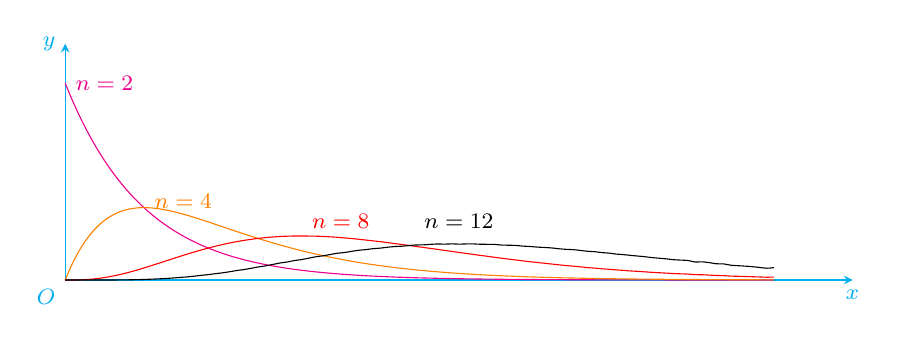
\begin{tikzpicture}[->,samples=100,>=stealth,font=\footnotesize,yscale=5,xscale=0.5]
        \def\xmin{0}
        \def\xmax{20}
        \def\ymin{0}
        \def\ymax{.6}
        \def\a{0.0104167}
        \def\b{0.000130208}
        
        \draw[->,cyan](\xmin,0)--(0,0)node[below left]{$O$}--(\xmax,0)node[below]{$x$};
        \draw[->,cyan](0,\ymin)--(0,\ymax)node[left]{$y$};
    
        \draw[domain=0:18,smooth,variable=\x,magenta,-] plot ({\x},{0.5*exp(-\x/2)}) node[magenta] at (1,0.5) {$n=2$};
        \draw[domain=0:18,smooth,variable=\x,orange,-] plot ({\x},{0.25*\x*exp(-\x/2)}) node[orange] at (3,0.2) {$n=4$};
        \draw[domain=0:18,smooth,variable=\x,red,-] plot ({\x},{\a*\x*\x*\x*exp(-\x/2)}) node[red] at (7,0.15) {$n=8$};
        \draw[domain=0:18,smooth,variable=\x,black,-] plot ({\x},{\b*\x*\x*\x*\x*\x*exp(-\x/2)}) node[black] at (10,0.15) {$n=12$};
    \end{tikzpicture}
    \caption{}
\end{figure}

\begin{theorem}
    若 $ X \sim \chi^{2}(n)$, 则
    $E(X)=n, D(X)=2 n .$
\end{theorem}

\begin{example}
    设 $X_1,x_2,\cdots,X_n,X_{n+1}$ 为总体 $X\sim N\qty(\mu,\sigma^2)$ 的简单随机样本, 且有 $$\bar{X}=\dfrac{1}{n}\displaystyle\sum_{i=1}^{n}X_i,~T=\dfrac{n}{(n+1)\sigma^2}\qty(X_{n+1}-\bar{X})^2$$
    求 $T$ 服从的分布, 并计算 $E(T)$ 和 $D(T)$.
\end{example}
\begin{errorSolution}
    由题意知 $X_{n+1}\sim N\qty(\mu,\sigma^2),~\bar{X}\sim N\qty(\mu,\dfrac{1}{n}\sigma^2)$, 且 $X_{n+1}$ 与 $\bar{X}$ 相互独立, 故 $X_{n+1}-\bar{X}\sim N\qty(0,\dfrac{n-1}{n}\sigma^2)$, \\
    \textbf{错因: }不能简单的加减法, 要从期望和方差的角度进行计算.\\
\end{errorSolution}
\begin{solution}
    由题意知 $X_{n+1}\sim N\qty(\mu,\sigma^2),~\bar{X}\sim N\qty(\mu,\dfrac{1}{n}\sigma^2)$, 且 $X_{n+1}$ 与 $\bar{X}$ 相互独立, 
    $$E\qty(X_{n+1}-\bar{X})=E(X_{n+1})-E\qty(\bar{X})=\mu-\mu=0,~D\qty(X_{n+1}-\bar{X})=D(X_{n+1})+D\qty(\bar{X})=\sigma^2+\dfrac{\sigma^2}{n}=\dfrac{n+1}{n}\sigma^2$$
    因此 $X_{n+1}-\bar{X}\sim N\qty(0,\dfrac{n+1}{n}\sigma^2)$, 则 $\dfrac{X_{n+1}-\bar{X}-0}{\sqrt{\dfrac{n+1}{n}}\sigma}\sim N(0,1)$, 两边平方有
    $$\qty(\dfrac{X_{n+1}-\bar{X}-0}{\sqrt{\dfrac{n+1}{n}}\sigma})^2=\dfrac{n}{(n+1)\sigma^2}\qty(X_{n+1}-\bar{X})^2=T\sim\chi^2(1)$$
    故 $E(T)=1,~D(T)=2.$
\end{solution}

\begin{theorem}[分布的可加性]
    设 $ X \sim \chi^{2}\left(n_{1}\right), Y \sim \chi^{2}\left(n_{2}\right) $, 且 $ X, Y $ 相互独立, 则
    $$X+Y \sim \chi^{2}\left(n_{1}+n_{2}\right) .$$
\end{theorem}

\begin{theorem}[$\chi^2$ 分布上 $ \alpha $ 分位点]
    设 $ \chi^{2} \sim \chi^{2}(n) $, 对于给定的 $ \alpha~~(0<\alpha<1) $, 满足条件
    $$P\left\{\chi^{2}>\chi_{\alpha}^{2}(n)\right\}=\int_{\chi_{\alpha}^{2}(n)}^{+\infty} f(y) \mathrm{d} y=\alpha$$
    的点 $ \chi_{\alpha}^{2}(n) $ 称为 $ \chi^{2}(n) $ 分布的上 $ \alpha $ 分位点.
\end{theorem}

\begin{example}
    已知 $(X,Y)$ 的概率密度函数为 $\displaystyle f(x,y)=\dfrac{1}{2\pi}\e^{-\frac{1}{2}\qty(x^2+y^2-2y+1)},-\infty<x,y<+\infty$, 求 $\dfrac{X^2}{(Y-1)^2}$ 服从的分布及参数.
\end{example}
\begin{solution}
    已知二维正态分布概率密度函数为 $$f(x,y)=\dfrac{1}{2\pi\sigma_1\sigma_2\sqrt{1-\rho^2}}\e^{-\frac{1}{2\qty(1-\rho^2)}\qty[\frac{(x-\mu_1)^2}{\sigma_1^2}-2\rho\frac{(x-\mu_1)(x-\mu_2)}{\sigma_1\sigma_2}+\frac{(y-\mu_2)^2}{\sigma_2^2}]}$$
    因此 $f(x,y)=\dfrac{1}{2\pi}\e^{-\frac{1}{2}\qty(x^2+y^2-2y+1)}\sim N(0,1;1,1;0)$, 故 $X\sim N(0,1),~Y\sim N(1,1)$ 且 $X,Y$ 相互独立, 那么 $\dfrac{X^2}{(Y-1)^2}\sim F(1,1).$
\end{solution}

\begin{example}
    设 $X_1,X_2$ 是来自总体 $X$ 的简单随机样本, 且 $\bar{X}=\dfrac{1}{2}\displaystyle \sum_{i=1}^{2}X_i,S_2^2=\sum_{i=1}^{2}\qty(X-\bar{X})^2,Y=\sqrt{X_1X_2}$, 
    \begin{enumerate}[label=(\arabic{*})]
        \item 若 $X$ 服从参数为 $\dfrac{1}{2}$ 的指数分布, 求 $EY$;
        \item 若 $X\sim N\qty(\mu,\sigma^2)$, 求 $E\qty[\qty(\bar{X}S_2^2)^2].$
    \end{enumerate}
\end{example}
\begin{solution}
    \begin{enumerate}[label=(\arabic{*})]
        \item $EY=E\qty(\sqrt{X_1X_2})=\qty[E\qty(\sqrt{X})]^2$, 下求 $E\sqrt{X}$, 
              \begin{flalign*}
                  E\sqrt{X}=\int_{-\infty}^{+\infty}\sqrt{x}\cdot f(x)\dd x=\int_{0}^{+\infty}\sqrt{x}\cdot\dfrac{1}{2}\e^{-\frac{1}{2}x}\dd x\xlongequal{\frac{1}{2}x=t}\sqrt{2}\int_{0}^{+\infty}\sqrt{t}\e^{-t}\dd t=\sqrt{2}\Gamma\qty(\dfrac{3}{2})=\dfrac{\sqrt{2}}{2}\Gamma\qty(\dfrac{1}{2})=\dfrac{\sqrt{2\pi}}{2}
              \end{flalign*}
              于是 $EY=\qty(\dfrac{\sqrt{2\pi}}{2})^2=\dfrac{\pi}{2}.$
        \item 因为 $\bar{X}$ 与 $S_2^2$ 相互独立, 所以
              \begin{flalign*}
                  E\qty[\qty(\bar{X}S_2^2)^2] & =E\qty(\bar{X}^2)E\qty[\qty(S_2^2)^2]=\qty[D\bar{X}+\qty(E\bar{X})^2]\qty[D\qty(S_2^2)+E^2\qty(S_2^2)]                        \\
                                              & =\qty[\dfrac{1}{n}DX+E^2X]\qty[\qty(\sigma^2)^2D\qty(\dfrac{S_2^2}{\sigma^2})+\qty(\sigma^2E\qty(\dfrac{S_2^2}{\sigma^2}))^2] \\
                                              & =\qty(\dfrac{1}{2}\sigma^2+\mu^2)\qty(2\sigma^4+\sigma^4)=3\sigma^4\qty(\dfrac{1}{2}\sigma^2+\mu^2).
              \end{flalign*}
    \end{enumerate}
\end{solution}

\subsection{\texorpdfstring{$t$}. 分布}

\begin{definition}[$t$ 分布]
    设随机变量 $ X \sim N(0,1), Y \sim \chi^{2}(n)$, 且 $ X, Y $ 相互独立, 则称随机变量
    $$T=\frac{X}{\sqrt{Y / n}}$$
    服从自由度为 $ n $ 的 $ t $ 分布, 记为 $ T \sim t(n) .$
\end{definition}

\begin{theorem}
    $ t $ 分布的概率密度函数 $ h(t) $ 为偶函数, 即 $ t_{1-\alpha}(n)=-t_{\alpha}(n) .$
\end{theorem}

\begin{theorem}
    当 $ n $ 足够大时, $t $ 分布近似于 $ N(0,1) $ 分布.
\end{theorem}
\begin{theorem}[$t$ 分布与 $F$ 分布]
    $ t^{2} \sim F(1, n) .$
\end{theorem}

\begin{definition}[$t $ 分布上 $ \alpha $ 分位点]
    设 $ t \sim t(n) $, 对于给定的 $ \alpha~~(0<\alpha<1) $, 满足条件
    $$P\left\{t>t_{\alpha}(n)\right\}=\int_{t_{\alpha}(n)}^{+\infty} h(t) \mathrm{d} t=\alpha$$
    的点 $ t_{\alpha}(n) $ 称为 $ t(n) $ 分布的上 $ \alpha $ 分位点.
\end{definition}

\subsection{\texorpdfstring{$F$}. 分布}

\begin{definition}[$F$ 分布]
    设随机变量 $ X \sim \chi^{2}\left(n_{1}\right), Y \sim \chi^{2}\left(n_{2}\right)$, 且 $ X, Y $ 相互独立, 则称随机变量
    $$F=\frac{X / n_{1}}{Y / n_{2}}$$
    服从自由度为 $ \left(n_{1}, n_{2}\right) $ 的 $ F $ 分布, 记为 $ F \sim F\left(n_{1}, n_{2}\right)$ .
\end{definition}

\begin{theorem}
    若 $ F \sim F\left(n_{1}, n_{2}\right) $, 则有 $ \dfrac{1}{F} \sim F\left(n_{2}, n_{1}\right) ,~F_{1-\alpha}\left(n_{1}, n_{2}\right)=\dfrac{1}{F_{\alpha}\left(n_{2}, n_{1}\right)}$.
\end{theorem}

\begin{theorem}[$F $ 分布上 $ \alpha $ 分位点]
    设 $ F \sim F\left(n_{1}, n_{2}\right) $, 对于给定的 $ \alpha(0<\alpha<1) $, 满足条件
    $$P\left\{F>F_{\alpha}\left(n_{1}, n_{2}\right)\right\}=\int_{F_{\alpha}\left(n_{1}, n_{2}\right)}^{+\infty} \psi(y) \mathrm{d} y=\alpha$$
    的点 $ F_{\alpha}\left(n_{1}, n_{2}\right) $ 称为 $ F\left(n_{1}, n_{2}\right) $ 分布的上 $ \alpha $ 分位点.
\end{theorem}

常用分布及其数学期望与方差.
\setcounter{magicrownumbers}{0}
\begin{table}[H]
    \centering
    \caption{常用分布及其数学期望与方差}
    \resizebox{.99\textwidth}{!}{
        \begin{tabular}{l l | c c}
            \textbf{分布名称及记号}                              & \textbf{概率函数或概率密度}                                                                                                                                                                                                                                                                    & \textbf{数学期望}             & \textbf{方差}                                             \\
            \toprule
            (\rownumber) “0-1” 分布                     & $p(x)=p^xq^{1-x},~x=0,1,~0<p<1,~p+q=1$                                                                                                                                                                                                                                                & $p$                  & $pq$                                             \\
            (\rownumber) 二项分布 $B(n,p)$              & $p(x)=\C_n^xp^xq^{n-x},~x=0,1,2,\cdots,n,~0<p<1,~p+q=1$                                                                                                                                                                                                                               & $np$                 & $npq$                                            \\
            (\rownumber) 超几何分布 $H(n,M,N)$          & $p(x)=\dfrac{\C_M^x\C_{N-M}^{n-x}}{\C_N^n},~x=0,1,\cdots,\min\qty{n,M},~0\leqslant n,M\leqslant N$                                                                                                                                                                                    & $\dfrac{nM}{N}$      & $\dfrac{nM(N-M)(N-n)}{N^2(N-1)}$                 \\
            (\rownumber) 泊松分布 $\pi(\lambda)$          & $p(x)=\dfrac{\lambda^x\e^{-\lambda}}{x!},~x=0,1,2,\cdots,~\lambda>0$                                                                                                                                                                                                                  & $\lambda$            & $\lambda$                                        \\
            (\rownumber) 几何分布 $G(p)$                & $p(x)=pq^{x-1},~x=1,2,\cdots,~0<p<1,~p+q=1$                                                                                                                                                                                                                                           & $\dfrac{1}{p}$       & $\dfrac{q}{p^2}$                                 \\
            \midrule
            (\rownumber) 均匀分布 $U(a,b)$              & $f(x)=\begin{cases}\dfrac{1}{b-1},&a\leqslant x\leqslant b\\0,&\text{其他}\end{cases}$                                                                                                                                                                                                & $\dfrac{a+b}{2}$     & $\dfrac{(b-a)^2}{12}$                            \\
            (\rownumber) 指数分布 $e(\lambda)$          & $f(x)=\begin{cases}\lambda\e^{-\lambda x},&x>0\\0,&\text{其他}\end{cases}\lambda>0$                                                                                                                                                                                                   & $\dfrac{1}{\lambda}$ & $\dfrac{1}{\lambda^2}$                           \\
            \midrule
            (\rownumber) 正态分布 $N\qty(\mu,\sigma^2)$ & $f(x)=\dfrac{1}{\sqrt{2\pi}\sigma}\e^{-\frac{(x-\mu)^2}{2\sigma^2}},~-\infty<x+\infty,~\sigma>0$                                                                                                                                                                                      & $\mu$                & $\sigma^2$                                       \\
            (\rownumber) $\chi^2$ 分布 $\chi^2(k)$      & $f(x)=\begin{cases}\dfrac{x^{\frac{k}{2}-1}\e^{-\frac{x}{2}}}{2^{\frac{k}{2}}\Gamma\qty(\dfrac{k}{2})},&x>0\\0,&x\leqslant 0\end{cases}k\in\mathbb{Z}$                                                                                         & $k$                  & $2k$                                             \\
            (\rownumber) $t$ 分布 $t(k)$                & $f(x)=\dfrac{\Gamma\qty(\dfrac{k+1}{2})}{\sqrt{k\pi}\Gamma\qty(\dfrac{k}{2})}\qty(1+\dfrac{x^2}{k})^{-\frac{k+1}{2}}$                                                                                                                                                                 & $0$                  & $\dfrac{k}{k-2}$                                 \\
            (\rownumber) $F$ 分布 $F(k_1,k_2)$          & $f(x)=\begin{cases}\dfrac{\Gamma\qty(\dfrac{k_1+k_2}{2})}{\Gamma\qty(\dfrac{k_1}{2})\Gamma\qty(\dfrac{k_2}{2})}k_1^{\frac{k_1}{2}}k_2^{\frac{k_2}{2}}\dfrac{x^{\frac{k_1}{2}-1}}{(k_1x+k_2)^{\frac{k_1+k_2}{2}}},&x>0\\0,&x\leqslant 0\end{cases}$ & $\dfrac{k_2}{k_2-2}$ & $\dfrac{2k_2^2(k_1+k_2-2)}{k_1(k_2-2)^2(k_2-4)}$
        \end{tabular}}
\end{table}

\begin{example}
    设 $X_1,X_2,\cdots,X_n~~(n\geqslant 2)$ 为来自总体 $N(\mu,1)$ 的简单随机样本, 及 $\bar{X}=\dfrac{1}{n}\displaystyle\sum_{i=1}^{n}X_i$, 则 不能得出结论
    \begin{tasks}(2)
        \task $\displaystyle \sum_{i=1}^{n}(X_i-\mu)^2$ 服从 $\chi^2$ 分布
        \task $\displaystyle 2(X_n-X_1)^2$ 服从 $\chi^2$ 分布
        \task $\displaystyle \sum_{i=1}^{n}\qty(X_i-\bar{X})^2$ 服从 $\chi^2$ 分布
        \task $\displaystyle n\qty(\bar{X}-\mu)^2$ 服从 $\chi^2$ 分布
    \end{tasks}
\end{example}
\begin{solution}
    $X_i-\mu\sim N(0,1)$, 由卡方分布的定义知 $\displaystyle\sum_{i=1}^{n}(X_i-\mu)^2\sim \chi^2(n)$, A 正确;
    $X_n\sim N(\mu,1),~X_1\sim N(\mu,1)$, 标准化处理有 $\dfrac{X_n-X_1}{\sqrt{2}}\sim N(0,1)$, 即 $\qty(\dfrac{X_n-X_1}{\sqrt{2}})^2\sim \chi^2(1)\Rightarrow \dfrac{\qty(X_n-X_1)^2}{2}\sim \chi^2(1)$, 故选项 B 错误;
    由于 $\displaystyle \sum_{i=1}^{n}\qty(X_i-\bar{X})^2=(n-1)S^2$, 而 $\dfrac{(n-1)S^2}{\sigma^2}\sim \chi^2(n-1)$, 则 $\dfrac{(n-1)S^2}{1}\sim \chi^2(n-1)$, 即 $\displaystyle \sum_{i=1}^{n}\qty(X_i-\bar{X})^2\sim \chi^2(n-1)$, C 正确;
    由于 $\dfrac{\bar{X}-\mu}{\sqrt{\dfrac{1}{n}}}\sim N(0,1)$, 则 $\displaystyle\qty(\dfrac{\bar{X}-\mu}{\sqrt{\dfrac{1}{n}}})^2=n\qty(\bar{X}-\mu)^2\sim \chi^2(1)$, D 正确.
\end{solution}

\begin{example}
    设 $X_1,X_2,\cdots,X_n$ 为来自正态总体 $N\qty(\mu,\sigma^2)$ 的简单随机样本, 则数学期望 $$E\qty{\displaystyle\qty(\sum_{i=1}^{n}X_i)\qty[\sum_{j=1}^{n}\qty(nX_j-\sum_{k=1}^{n}X_k)^2]}$$ 等于
    \begin{tasks}(4)
        \task $n^3(n-1)\mu\cdot\sigma^2$
        \task $n^2(n-1)\mu\cdot\sigma^2$
        \task $n(n-1)\mu\cdot\sigma^2$
        \task $n^3(n-1)\mu\cdot\sigma$
    \end{tasks}
\end{example}
\begin{solution}
    令 $\bar{X}=\dfrac{1}{n}\displaystyle\sum_{i=1}^{n}X_i$, 那么 $\displaystyle\sum_{i=1}^{n}X_i=n\bar{X}$, 
    $$\sum_{j=1}^{n}\qty(nX_j-\sum_{k=1}^{n}X_k)^2=\sum_{j=1}^{n}\qty(nX_j-n\bar{X})^2=n^2\sum_{j=1}^{n}\qty(X_j-\bar{X})^2=n^2(n-1)S^2$$
    因此
    $$E\qty{\displaystyle\qty(\sum_{i=1}^{n}X_i)\qty[\sum_{j=1}^{n}\qty(nX_j-\sum_{k=1}^{n}X_k)^2]}=E\qty[n\bar{X}\cdot n^2(n-1)S^2]=n^3(n-1)E\qty(\bar{X}\cdot S^2)\xlongequal{\bar{X},S^2\text{ 相互独立}}n^3(n-1)\mu\sigma^2$$
    故选 A.
\end{solution}

\begin{example}
    已知 $(X,Y)$ 的概率密度函数为 $\displaystyle f(x,y)=\dfrac{1}{2\pi}\e^{-\frac{1}{2}\qty(x^2+y^2-2y+1)},-\infty<x,y<+\infty$, 求 $\dfrac{X^2}{(Y-1)^2}$ 服从的分布及参数.
\end{example}
\begin{solution}
    已知二维正态分布概率密度函数为 $$f(x,y)=\dfrac{1}{2\pi\sigma_1\sigma_2\sqrt{1-\rho^2}}\e^{-\frac{1}{2\qty(1-\rho^2)}\qty[\frac{(x-\mu_1)^2}{\sigma_1^2}-2\rho\frac{(x-\mu_1)(x-\mu_2)}{\sigma_1\sigma_2}+\frac{(y-\mu_2)^2}{\sigma_2^2}]}$$
    因此 $f(x,y)=\dfrac{1}{2\pi}\e^{-\frac{1}{2}\qty(x^2+y^2-2y+1)}\sim N(0,1;1,1;0)$, 故 $X\sim N(0,1),~Y\sim N(1,1)$ 且 $X,Y$ 相互独立, 那么 $\dfrac{X^2}{(Y-1)^2}\sim F(1,1).$
\end{solution}

\begin{example}
    设总体 $X\sim N(0,1),~(X_1,X_2,\cdots,X_{10})$ 为 $X$ 的简单随机样本, 
    \begin{enumerate}[label=(\arabic{*})]
        \item 若 $T=\displaystyle\dfrac{1}{3}\qty(\sum_{i=1}^{3}X_i)^3+\dfrac{1}{7}\qty(\sum_{i=4}^{10}X_i)^2$, 求 $T$ 服从的分布;
        \item 若 $T=\dfrac{\displaystyle7\sum_{i=1}^{3}X_i^2}{\displaystyle 3\sum_{i=4}^{10}X_i^2}$, 求 $T$ 服从的分布;
        \item 若 $T=\dfrac{3X_1}{\sqrt{\displaystyle\sum_{i=2}^{10}X_i^2}}$, 求 $T$ 服从的分布.
    \end{enumerate}
\end{example}
\begin{solution}
    \begin{enumerate}[label=(\arabic{*})]
        \item 因为 $\displaystyle\sum_{i=1}^{3}X_i=X_1+X_2+X_3\sim N(0+0+0,1+1+1)=N(0,3)$, 所以
              $$\dfrac{1}{3}\qty(\sum_{i=1}^{3}X_i)^2=\dfrac{\displaystyle\qty(\sum_{i=1}^{3}X_i)^2}{\qty(\sqrt{3})^2}=\qty(\dfrac{\displaystyle\sum_{i=1}^{3}X_i-0}{\sqrt{3}})^2\sim \chi^2(1)$$
              同理 $\dfrac{1}{7}\qty(\displaystyle\sum_{i=4}^{10}X_i)^2=\dfrac{\qty(\displaystyle\sum_{i=4}^{10}X_i)^2}{\qty(\sqrt{7})^2}=\qty(\dfrac{\displaystyle\sum_{i=4}^{10}X_i-0}{\sqrt{7}})^2\sim\chi^2(1)$, 
              于是 $T=\displaystyle\dfrac{1}{3}\qty(\sum_{i=1}^{3}X_i)^3+\dfrac{1}{7}\qty(\sum_{i=4}^{10}X_i)^2\sim\chi^2(2).$
        \item $T=\dfrac{\displaystyle7\sum_{i=1}^{3}X_i^2}{\displaystyle 3\sum_{i=4}^{10}X_i^2}=\dfrac{\dfrac{\sum_{i=1}^{3}X_i^2}{3}}{\dfrac{\sum_{i=4}^{10}X_i^2}{7}}\sim F(3,7).$
        \item $T=\dfrac{3X_1}{\sqrt{\displaystyle\sum_{i=2}^{10}X_i^2}}=\dfrac{X_1}{\dfrac{\sqrt{\sum_{i=2}^{10}X_i^2}}{3}}=\dfrac{X_1}{\sqrt{\dfrac{\sum_{i=2}^{10}X_i^2}{9}}}\sim t(9).$
    \end{enumerate}
\end{solution}
